\documentclass[12pt]{article}
\usepackage[utf8]{inputenc}
\usepackage{longtable}
\usepackage{multirow}
\usepackage{graphicx}
\graphicspath{ {./author/} }


\renewcommand{\baselinestretch}{1.5}

\title{Harold V. McIntosh (1929-2015)}
\author{Luis Diego Jiménez Delgado}
\date{Agosto 13 del 2019}

\begin{document}

\maketitle

\begin{center}
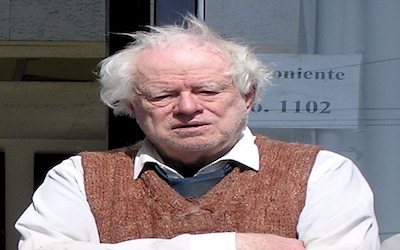
\includegraphics{m}
\end{center}
Uno de los grandes pioneros de la computación en el mundo y de los académicos más influyentes en la historia de esta ciencia en México, cuyo desarrollo está estrechamente ligado a su nombre, es también el hombre que echó por tierra cánones culturales para vivir la libertad del conocimiento, que sólo desde la soledad es posible ejercer en plenitud.
Originario de Denver, Colorado, en 1975 ingresó al Departamento de Aplicación de Microcomputadoras, del Instituto de Ciencias de la BUAP, espacio que fue responsable de ensamblar las primeras computadoras que tuvo la Institución, a la cual profesó gran cariño y dedicó sus últimos 42 años a la noble tarea de enseñar a múltiples generaciones de estudiantes.
Su amor por la ciencia y talento académico bien pueden ilustrarse con la cita de Gerardo Cisneros, en “La computación en México y la influencia de H.V. McIntosh en su desarrollo”, donde cita la entrevista a Sheldon Lee Glashow, publicada en The Atlantic Monthly en 1984, en la que el Premio Nobel de Física 1979 aseguró “que lo que aprendió de McIntosh sobre Teoría de Grupos en sus años de estudiante de licenciatura en Cornell, fue tanto o más importante que lo aprendido en curso alguno que hubiera tomado”.
Otros ejemplos de su gran influencia: entre otras tesis, dirigió la de licenciatura de Arturo Cisneros Stoianowski, que produjo tres artículos en Journal of Mathematical Physics; y las de J. Leonel Torres Hernández y Jesús Ortega Campos, premiados por la Sociedad Mexicana de Física. De 1964 a 1965, las de Adolfo Guzmán Arenas y Raymundo Segovia Navarro, sobre compiladores para el lenguaje de programación Convert, ideado por McIntosh para realizar manipulaciones simbólicas útiles en la solución de problemas de mecánica clásica y cuántica, hoy personalidades ampliamente reconocidas en su campo.
José Luis Meza León, académico de la Facultad de Ciencias de la Computación de la BUAP y uno de sus más cercanos amigos, destaca que su llegada a México, cuya estancia inició en 1961, para impartir unas conferencias en la UNAM, “resultó todo un beneficio, pues fue el personaje que llegó para ser pilar del desarrollo de la computación en nuestro país, y Puebla la ciudad a la que mayores beneficios legó, al ser uno de los fundadores del Colegio de Computación de la Universidad Autónoma de Puebla, hoy BUAP”.
\\
\textbf{Refencias:}
[1]Genaro J. Mart ́ınez1,2, Juan C. Seck-Tuoh-Mora3 Sergio V. Chapa-Vergara4, Christian Lemaitre 5(2019) Brief Notes and History Computing in Mexico during 50 years∗, https://arxiv.org/pdf/1905.07527.pdf

\end{document}